\chapter{Contexto}
\label{chap:contexto}

\lettrine{N}{este} apartado introdúcese o contexto relevante a este traballo que provee os conceptos básicos necesarios para a súa comprensión.
Para elo descríbese o campo da oftalmoloxía e a imaxe médica, así como o estado da arte en aliñamento de imaxes.
\section{Oftalmoloxía}
\label{sec:Oftalmoloxía}
A oftalmoloxía é a especialidade médica encargada do estudo e tratamento das enfermidades dos ollos, incluíndo o globo ocular, a súa musculatura, o sistema lagrimal e as pálpebras.
O ollo humano é un dos órganos dos que máis dependemos e maior cantidade de información sensorial aporta, así como un dos máis complexos do noso corpo \cite{kanski2011clinical}.

A importancia da oftalmoloxía radica non só no tratamento das enfermidades oculares, senón tamén na súa capacidade para proporcionar información valiosa sobre o estado de saúde xeral do paciente. 
A observación directa dos vasos sanguíneos e do tecido neuronal 'in vivo' permite aos oftalmólogos detectar signos precoces de diversas enfermidades sistémicas.
 Por exemplo, o glaucoma, que non presenta síntomas nas súas etapas iniciais, pode ser diagnosticado mediante exames regulares da presión ocular e do nervio óptico \cite{importglaucoma}.
 Esta capacidade de diagnóstico precoz fai da oftalmoloxía unha especialidade fundamental na prevención e no mantemento da saúde visual e xeral do paciente.

 \subsection{Anatomía do ollo humano}
\label{subsec:Anatomía do ollo humano}
O ollo encargase de captar a luz e transformala en impulsos eléctricos que se envían ao cerebro.
 Esta información é interpretada polo cerebro, que mediante mecanismos como a atención e a memoria, permite a percepción visual. \cite{eyefunct}
 O ollo humano está composto por varias estruturas, cada unha cunha función específica que permite a percepción visual \cite{eyeanat}. Entre elas destacan:

 \begin{itemize}
 \item Córnea e Cristalino: actúan xuntas para enfocar a luz na retina. A córnea, situada na parte exterior do ollo, proporciona maior parte da capacidade refractiva, mentres que o cristalino, unha lente flexible, axusta o enfoque para obxectos a diferentes distancias.
 \item Pupila e Iris: regulan a cantidade de luz que entra no ollo. O iris, a parte coloreada do ollo, expándese ou contráese para controlar o tamaño da pupila, o orificio central.
 \item Retina: unha capa de células sensibles á luz (fotorreceptores) que converten os estímulos luminosos en sinais eléctricas, procesados inicialmente na retina mesma.
 \item Nervio óptico: transporta as sinais eléctricas xeradas na retina ata o cerebro, onde se interpretan como imaxes.
 \item Disco óptico: tamén coñecido como "punto cego", é a área onde o nervio óptico sae do ollo; carece de fotorreceptores.
 \item Vasos sanguíneos: distribúen os nutrientes e o osíxeno necesarios á retina e eliminan os seus residuos metabólicos.
 \end{itemize}

A figura \ref{fig:imaxes_ojo} mostra estas estruturas localizadas en imaxes.

\begin{figure}[tbp]
    \centering
    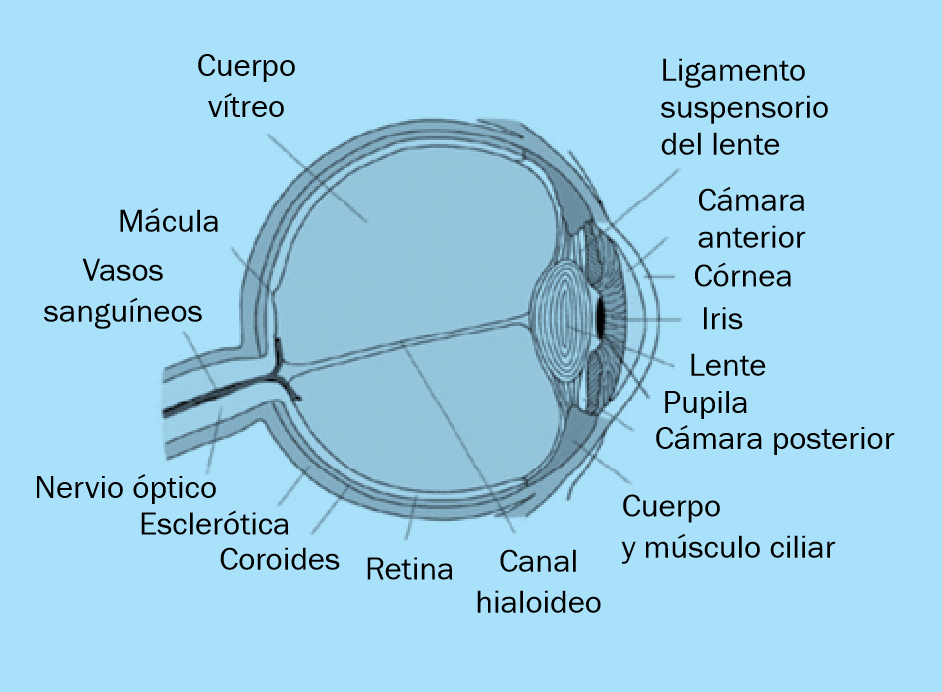
\includegraphics[width=0.45\textwidth]{imaxes/ojo1.png}
    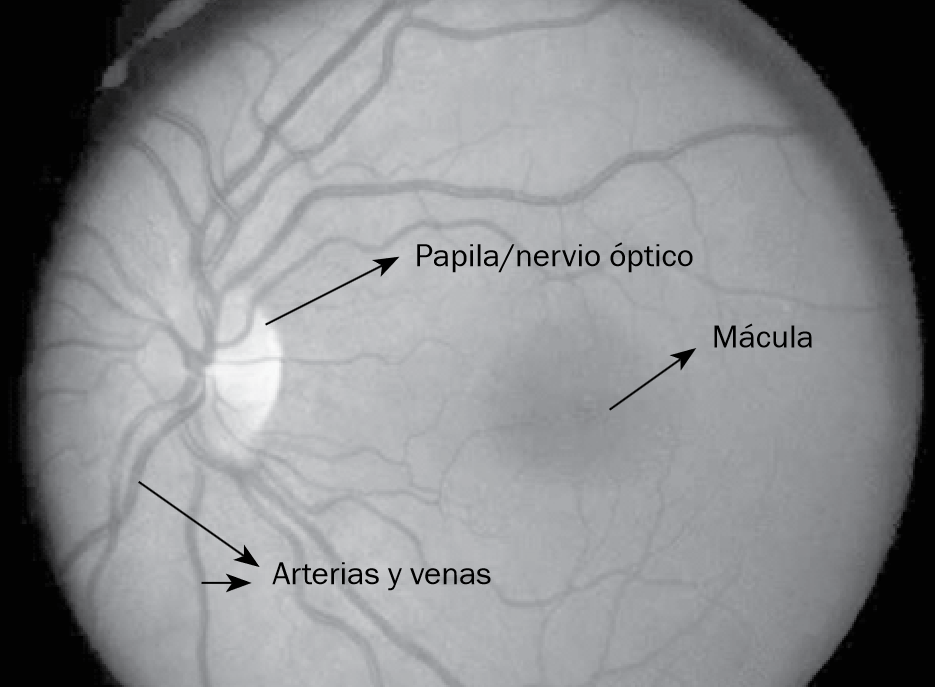
\includegraphics[width=0.45\textwidth]{imaxes/ojo2.png}
    \caption{Imaxes do ollo humano, extraídas de \cite{visionyojo}. Á esquerda, vista lateral do ollo anotada. Á dereita, retinografía do ollo anotada.}
    \label{fig:imaxes_ojo}
\end{figure}

\subsection{Imaxe oftalmolóxica}
\label{subsec:Imaxe oftalmolóxica}
Existen diversas modalidades de imaxe médica que permiten observar o ollo, cada unha con diferentes propiedades e aplicacións. 
Entre elas inclúense a fotografía de fondo de ollo, a tomografía de coherencia óptica (OCT) e a angiografía con fluoresceína \cite{ilginis2014ophthalmic}.

Este traballo céntrase na fotografía de fondo de ollo entre outras razóns polo seu uso común na práctica clínica.
Isto é débese en gran parte á súa accesibilidade, requerindo equipo maís barato e menor adestramento comparada cas outras modalidades. 
Ademais, é unha técnica non invasiva e rápida de realizar, o que a fai preferible na maioría dos casos \cite{retinimaging}.

Para realizala faise uso dunha cámara especial denominada retinógrafo, e xeralmente require da previa dilatación da pupila do paciente.
Desta forma permítese maior entrada de luz nos ollos, o que provoca unha mellor visualización da retina e mellora a calidade da imaxe.
Un especialista pode analizar a retinografía para detectar signos de enfermidades como a retinopatía diabética, a hipertensión ou a dexeneración macular \cite{retreggood}.

\section{Rexistro de imaxes}
\label{sec:Rexistro de imaxes}
O rexistro de imaxes é un proceso que consiste en, sobre dúas ou máis imaxes, determinar a correspondencia espacial entre elas
 e alinealas nun sistema de coordenadas común, co obxetivo de que as características de interese se atopen na mesma posición.

% Por exemplo, no caso do stitching de fotografías panorámicas, o rexistro de imaxes permite identificar correspondencias entre puntos característicos en múltiples tomas solapadas
%  e axustar a súa posición relativa nun marco común. Esta etapa é necesaria para a posterior fusión das imaxes, de modo que as distintas vistas se aliñen con precisión, producindo un resultado final continuo e sen irregularidades visuais.

O rexistro de imaxes ten utilidade en moitos campos diferentes como a imaxe satelital, xeografía, robótica... mais o 
campo da imaxe médica é dos máis interesantes póla súa aplicación práctica e é o que se aborda neste traballo \cite{goshtasby2017theory}.
Estas imaxes poden variar a nivel temporal, espacial, de dimensión ou de modalidade.

No ámbito da saúde un rexistro adecuado pode empregarse para comparar imaxes dun mesmo paciente tomadas en distintos momentos, en distintas modalidades ou para comparar entre diferentes pacientes.
Isto permite a revisión do avance dunha enfermidade ao longo do tempo, a fusión de imaxes de distintas modalidades ou a detección de patróns comúns entre distintos individuos.
A fusión de imaxes permite interpretar moito mellor a información dispoñible nelas, e é de gran axuda para guiar aos médicos na toma de decisións.
Tamén é útil para correxir os movementos involuntarios do paciente durante a adquisición de imaxes, como no caso da respiración en imaxes de pulmóns, ou para a intervención guiada por imaxe (\gls{IGRT}) que non 
podería funcionar sen a utilización axeitada de técnicas de rexistro de imaxes \cite{wang2022neuralrenderingstereo3d}. 

Ata recentemente, gran parte do traballo de rexistro facíase de forma manual por expertos con software como BigWarp \cite{bigwarp}, 
e dependía das habilidades do profesional para detectar as características de interese e realizar o aliñamento.
Isto facía que o proceso fose lento e propenso a erros, ademais de pouco práctico para grandes volumes de imaxes.

Na figura \ref{fig:retin_reg} móstrase un exemplo de rexistro de imaxes de retina, onde se pode observar como as imaxes son aliñadas para que as estruturas anatómicas coincidan.

\begin{figure}[tbp]
    \centering
    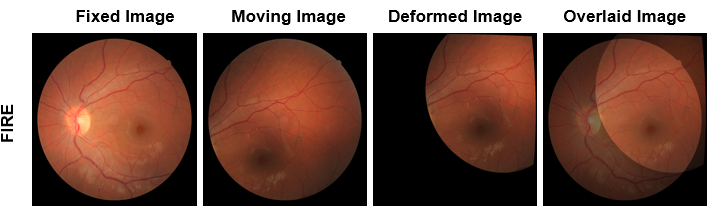
\includegraphics[width=0.8\textwidth]{imaxes/retin-reg.png}
    \caption{Exemplo de rexistro de imaxes de retina \cite{sivaraman2024retinaregnetzeroshotapproachretinal}}
    \label{fig:retin_reg}
\end{figure}

\subsection{Categorías de rexistro}
\label{subsec:Categorías de rexistro}

% O rexistro de imaxes pode ser clasificado en distintas categorías segundo as súas características. Na figura \ref{fig:categorias_de_rexistro} un resumo móstranse das categorías mais comúns.
O rexistro de imaxes pode ser clasificado en distintas categorías segundo as súas características.
% \begin{figure}[hp!]
%     \centering
%     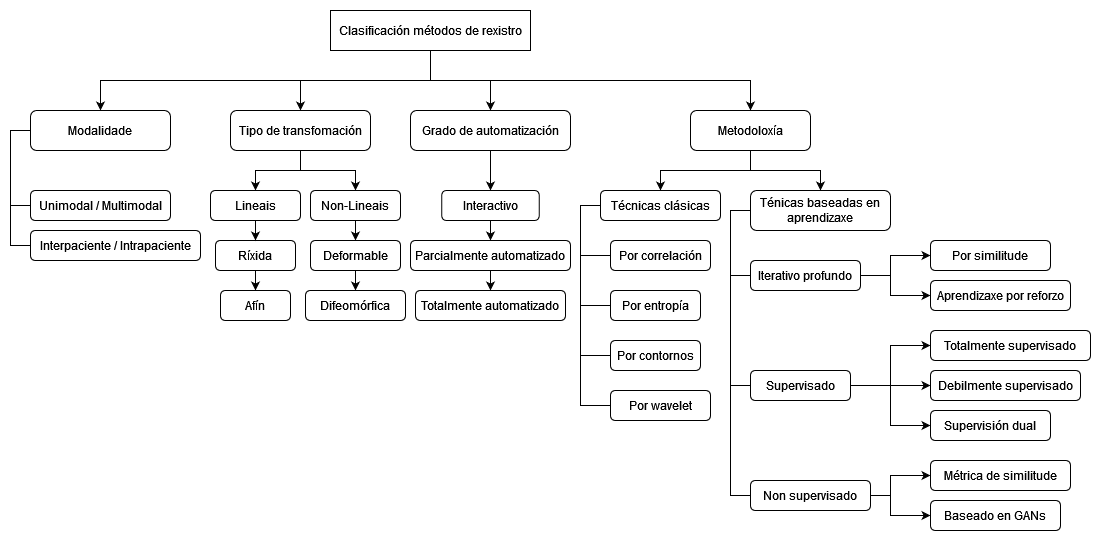
\includegraphics[width=1\textwidth]{imaxes/catreg.drawio.png}
%     \caption{Categorías de rexistro}
%     \label{fig:categorias_de_rexistro}
% \end{figure}

\begin{itemize}
    \item \textbf{Segundo o número de imaxes:}
    \begin{itemize}
        \item \textit{Par a par:} O rexistro realízase entre dúas imaxes, unha fixa e unha móbil.
        \item \textit{Múltiple:} Rexístranse varias imaxes simultaneamente, buscando unha correspondencia global.
    \end{itemize}

    \item \textbf{Segundo a modalidade:}
    \begin{itemize}
        \item \textit{Intra-modalidade:} As imaxes pertencen á mesma modalidade (por exemplo, dúas retinografías).
        \item \textit{Inter-modalidade:} As imaxes proveñen de modalidades diferentes (por exemplo, retinografía e OCT).
    \end{itemize}

    \item \textbf{Segundo o tipo de transformación:}
    \begin{itemize}
        \item \textit{Ríxida:} Só permite traslación e rotación, mantendo as distancias e ángulos.
        \item \textit{Afín:} Ademais de traslación e rotación, permite escalado e cizallamento.
        \item \textit{Deformable (non ríxida):} Permite deformacións locais complexas e non lineais.
        \item \textit{Difeomórfica:} Transformación non ríxida que é continua, invertible e diferenciable en todo o seu dominio. Se non ten esta característica, non se pode garantir que a transformación sexa reversíbel, polo que son preferidas en moitos casos \cite{han2022diffeomorphicimageregistrationneural}.
    \end{itemize}

    \item \textbf{Segundo o grao de automatización:} \cite{deeplernreview3dreg}
    \begin{itemize}
        \item \textit{Manual:} O usuario selecciona puntos de control ou axusta parámetros.
        \item \textit{Automático:} O proceso realízase sen intervención humana, mediante algoritmos.
        \item \textit{Semiautomático:} Combina intervención manual e automática.
    \end{itemize}

    \item \textbf{Segundo a natureza da transformación:}
    \begin{itemize}
        \item \textit{Simétrico:} A transformación é consistente en ambas direccións entre as imaxes.
        \item \textit{Asimétrico:} A transformación calcúlase só nun sentido. Cando se traballa con imaxes de forma asimétrica, a imaxe de referencia denomínase imaxe fixa e a imaxe que se quere rexistrar imaxe móbil.
    \end{itemize}

\end{itemize}

% \begin{itemize}
%     \item \textbf{Metodoloxía}
%     \begin{itemize}
%         \item \textbf{Técnicas clásicas} \cite{zitova2003imageregistrationsurvey}
%         \begin{itemize}
%             \item \textit{Por correlación:} Optimizan funcións de correlación entre as intensidades das imaxes para atopar a mellor aliñación.
%             \item \textit{Por entropía:} Baseados na maximización da información mutua, resultan especialmente útiles en rexistro multimodal.
%             \item \textit{Por contornos:} Empregan características xeométricas, como bordes ou liñas estruturais, para establecer correspondencias espaciais.
%             \item \textit{Por wavelet:} Utilizan descomposicións en diferentes frecuencias e resolucións para capturar información relevante.
%         \end{itemize}
        
%         \item \textbf{Técnicas baseadas en aprendizaxe} \cite{deeplernreview3dreg, bharati2022deeplearningmedicalimage}
%         \begin{itemize}
%             \item \textit{Iterativo profundo:} Estratexias que aplican redes neurais de forma recursiva para refinar progresivamente a transformación estimada.
            
%             \item \textbf{Aprendizaxe supervisada}
%             \begin{itemize}
%                 \item \textit{Totalmente supervisado:} Require datos de adestramento con aliñacións precisas (ground truth), que permiten optimizar directamente a tarefa de rexistro.
%                 \item \textit{Debilmente supervisado:} Emprega información parcial ou indirecta, como anotacións espaciais limitadas ou métricas proxy.
%                 \item \textit{Supervisión dual:} Combina diferentes formas de supervisión, como etiquetas explícitas e funcións de perda auto-supervisadas, para aumentar a xeneralización.
%             \end{itemize}
            
%             \item \textbf{Aprendizaxe non supervisada}
%             \begin{itemize}
%                 \item \textit{Métrica de similitude:} Optimiza criterios de similitude (e.g., NCC, SSIM) sen necesidade de datos anotados, favorecendo adaptación a novos dominios.
%                 \item \textit{Baseado en GANs:} Emprega arquitecturas adversarias para aprender transformacións realistas entre imaxes sen supervisión directa.
%             \end{itemize}
            
%             \item \textit{Por similitude:} Modelos que aprenden funcións de custo diferenciables que maximizan a coincidencia entre as imaxes de entrada.
%             \item \textit{Aprendizaxe por reforzo:} Formula o rexistro como un problema de toma de decisións, onde un axente aprende políticas óptimas mediante retroalimentación ambiental.
%         \end{itemize}
%     \end{itemize}
% \end{itemize}

As transformacións lineais globais soen representanse en matrices de transformación, onde cada elemento da matriz representa un parámetro da transformación.

No caso de transformacións máis complexas, utilízanse campos de vectores de deformación (\gls{DFV}s), que permite representar deformacións locais na imaxe, facendoa moito máis flexible para representar transformacións non lineais e detalladas.
Os DFVs adoitan ser representados cunha matriz de igual tamaño á imaxe, onde cada elemento representa un vector que indica a dirección e a magnitude da deformación.

Este traballo ubícase no rexistro de imaxes par a par, intra-modaliade e con transformacións deformables. É un proceso totalmente automático que produce transfomacións asimétricas.

Na figura \ref{fig:dfv_visualization} móstranse dúas formas de visualizar un DFV: mediante frechas que indican a dirección e magnitude da deformación, e aplicando a deformación a unha cuadrícula para ver como se distorsiona.

\begin{figure}[tbp]
    \centering
    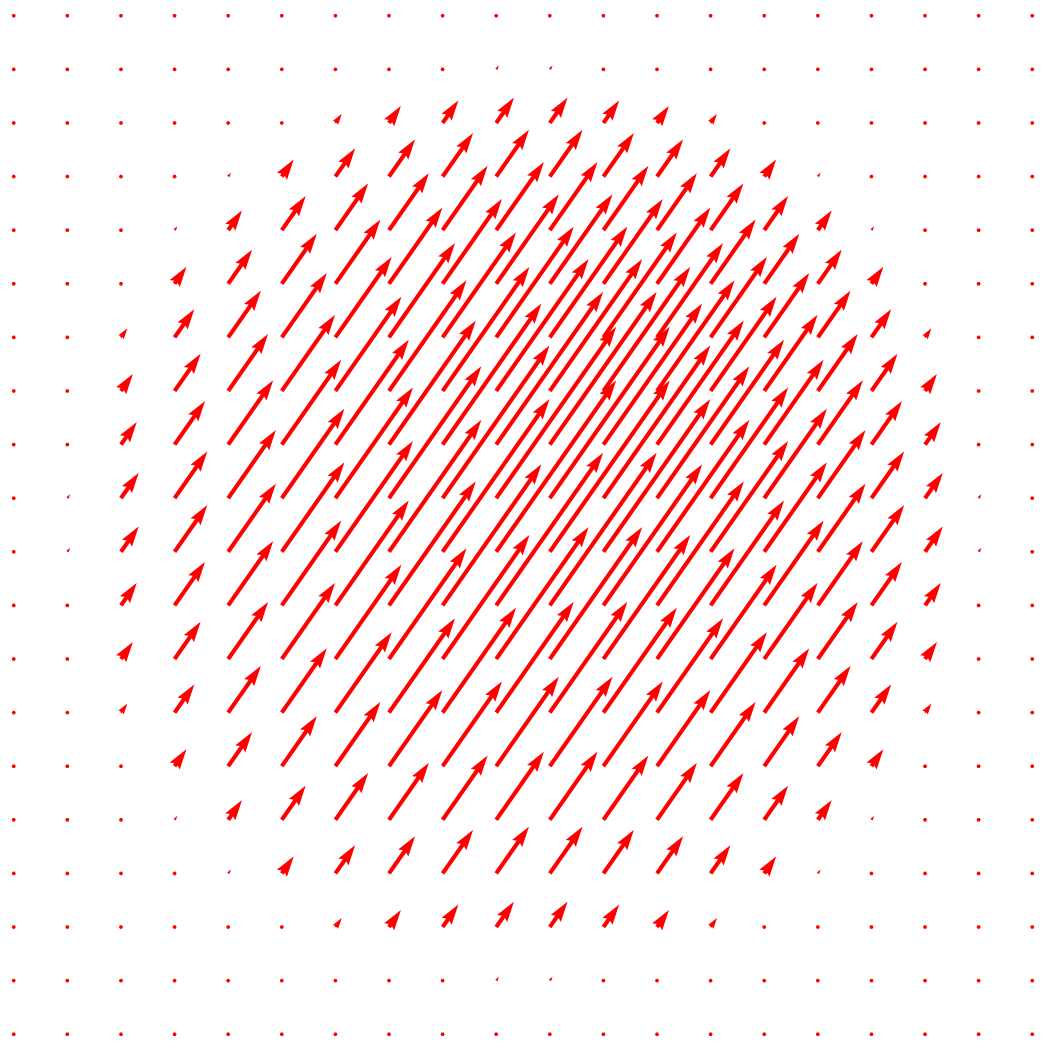
\includegraphics[width=0.45\textwidth]{imaxes/dfv_arrows.png}
    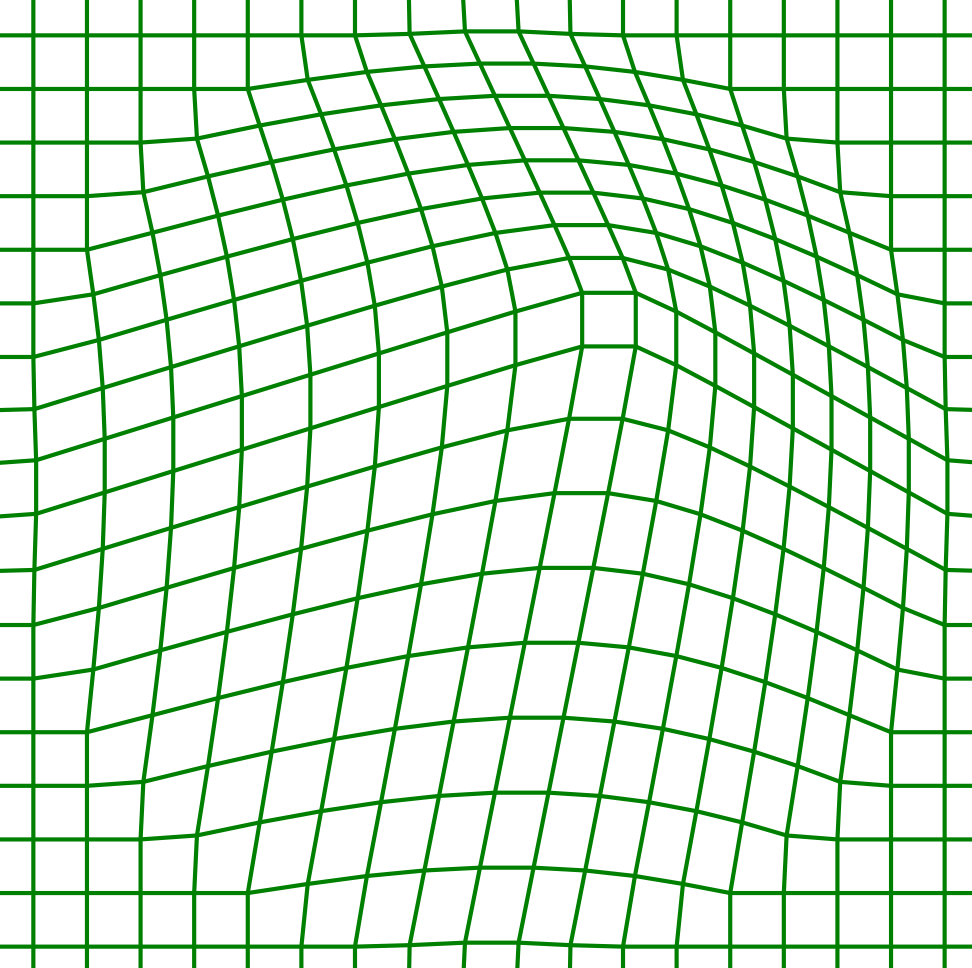
\includegraphics[width=0.45\textwidth]{imaxes/dfv_grid.png}
    \caption{Visualización do campo de vectores de deformación (DFV). Á esquerda, representación mediante frechas. Á dereita, esta deformación aplicada a unha cuadrícula.}
    \label{fig:dfv_visualization}
\end{figure}

\subsection{Estado da arte}
\label{subsec:Estado da arte}

% Pese á gran cantidade de avances que está a ocorren no campo do aprendizaxe profunda, os métodos clásicos de rexistro de imaxes seguen a ser o estado do arte na maioría de casos,
% principalmente debido á importancia da precisión e a robustez en imaxe médica.

O rexistro de imaxes médicas constitúe unha área de investigación fundamental que experimentou importantes avances nas últimas décadas. Neste ámbito, a precisión e a robustez do rexistro cobran especial relevancia, xa que son empregados para o diagnóstico e seguimento de enfermidades, así como para a planificación de tratamentos cirúrxicos.
No eido da oftalmoloxía, os métodos que funcionan ben en varios dominios de imaxe médica (cerebro, pulmóns, etc) adoitan requirir de axustes para funcionar en retinas, polo que hai un estado da arte paralelo. 

A evolución dos métodos de rexistro en retinografías reflicte a transición dende enfoques puramente algorítmicos cara metodoloxías híbridas, onde publicacións recentes como HybridRetina \cite{liu2024progressiveretinalimageregistration}  mostran como para acadar os mellores resultados é beneficioso combinar ambos enfoques, aproveitando a precisión dos métodos clásicos e a adaptabilidade dos métodos de aprendizaxe automático.

\subsubsection{Métodos clásicos}
\label{subsubsec:Métodos clásicos}

Os métodos clásicos de rexistro de imaxes médicas poden clasificarse en dúas categorías principais:
Aqueles baseados en similitude de imaxe (\gls{IBR}) e aqueles baseados en características (\gls{FBR}).
Tamén existen métodos híbridos que combinan ambos enfoques \cite{integrateintfeat}.
O resultado final pode ser os parámetros da transformación ou a imaxe fusionada.

\paragraph{Métodos baseados en similitude de imaxe}
\label{par:Métodos baseados en similitude de imaxe}

O rexistro realízase comparando os valores de intensidade dos píxeles ou voxeles mediante unha métrica de similitude entre a imaxe fixa e a imaxe móbil.
Este enfoque tende a requerir de múltiples iteracións para converxer, nas cales calcúlase o grado de semellanza entre as imaxes e
actualízanse os parámetros da transformación utilizando un mecanismo de optimización ata que se cumpran os criterios de terminación.

Os métodos de rexistro tradicionais teñen tres compoñentes principais: a métrica de similitude, o optimizador e o modelo de transformación. 

A figura \ref{fig:rexistro_iterativo} mostra un diagrama do proceso de rexistro iterativo.

% ejemplos?

\paragraph{Métodos baseados en características}
\label{par:Métodos baseados en características}

O rexistro realízase identificando e emparellando características salientables entre as imaxes, como puntos, liñas ou bordes.
Tipicamente, estes métodos teñen 3 pasos principais:

\begin{itemize}
\item \textbf{Detección de puntos de interese:} Identificación de puntos ou rexións salientables nas imaxes, como bordes, esquinas ou texturas. Para isto poden utilizarse utilízanse algoritmos como SIFT \cite{sift}, SURF \cite{surf}, BRISK \cite{brisk} ou FREAK \cite{freakkeypoint}.
\item \textbf{Descrición de características:}  os puntos detectados son descritos e comparados entre imaxes usando descritores .
\item \textbf{Estimación da transformación:} unha vez atopadas as correspondencias, calcúlase a transformación que aliña as imaxes con algoritmos de emparellamento como FLANN \cite{flann} ou RANSAC \cite{ransac}.
\end{itemize}

Algúns dos métodos tradicionalmente máis utilizados neste campo son \gls{GDB-ICP} \cite{GDB-ICP} e Harris-PIIFD \cite{piifd}. Este último utiliza o algoritmo Harris \cite{Harris1988ACC} para a detección de puntos de interese, descríbenos con \gls{PIIFD}, e emparéllanse usando \gls{BBF} \cite{BBF}.
 Finalmente, refínanse as coincidencias e escóllese a transformación (ríxida, afín ou polinomial) segundo o número de pares de puntos válidos. Sobre esta base propuxéronse varias melloras para adaptalo ao rexistro multimodal de retinas como UR-SIFT \cite{ur-sift} ou \gls{GMM} \cite{GMM}.

Unha vantaxe deste enfoque é a capacidade para rexistrar imaxes con grandes variacións locais ou modalidades diferentes, xa que non depende tanto da semellanza global entre as imaxes.

Outros métodos clásicos relevantes no campo da imaxe de ollo inclúen REMPE \cite{rempe}, que estima simultaneamente a pose das cámaras e a forma do ollo. Fai uso de un modelo elipsoidal para o ollo e estima a posición das cámaras con RANSAC, para logo refinala cunha variante de PSO \cite{pso}. 
% Versións anteriores deste método utilizaron modelos esféricos e \gls{SURF} no canto de SIFT \cite{H-M16}.

\begin{figure}[tbp]
\centering
\begin{tikzpicture}[node distance=2cm, scale=0.8, every node/.style={transform shape}]
% Nodes
\node (imageFixa) [process] {Imaxe Fixa};
\node (imageMobil) [process, right of=imageFixa, xshift=3cm] {Imaxe Móbil};
\node (featureExtraction) [process, below of=imageFixa, yshift=-1cm] {Cálculo de medida de similitude};
\node (parameterUpdate) [process, below of=featureExtraction, yshift=-1cm] {Actualización de Parámetros};
\node (applyTransformation) [process, below of=parameterUpdate, yshift=-1cm] {Aplicar a Transformación};
\node (criteriaCheck) [decision, below of=applyTransformation, yshift=-1cm] {Criterios Cumpridos?};
\node (result) [process, below of=criteriaCheck, yshift=-1cm] {Resultado};
% Arrows
\draw [arrow] (imageFixa) -- (featureExtraction);
\draw [arrow] (imageMobil) -- (featureExtraction);
\draw [arrow] (featureExtraction) -- (parameterUpdate);
\draw [arrow] (parameterUpdate) -- (applyTransformation);
\draw [arrow] (applyTransformation) -- (criteriaCheck);
\draw [arrow] (criteriaCheck) -- node[anchor=west] {Sí} (result);
\draw [arrow] (criteriaCheck.east) -- ++(1,0) node[anchor=south, xshift=0.5cm] {No} |- (featureExtraction.east);
\end{tikzpicture}
\caption{Proceso de rexistro de imaxes iterativo}
\label{fig:rexistro_iterativo}
\end{figure}

Tamén existen múltiples programas que fan uso de estos métodos en ferramentas para facilitar o rexistro de imaxes, como SimpleITK \cite{simpleitk}, Elastix \cite{elastix} ou ANTs \cite{ants}.

\subsubsection{Métodos de aprendizaxe profunda}
\label{subsubsec:Métodos de aprendizaxe profunda}

Ca chegada dos métodos de aprendizaxe profunda á imaxe médica, comezaron a empregarse redes neuronais para realizar o aliñamento de imaxes.
Existe un gran interés polos métodos baseados en aprendizaxe profundo, como se reflexa no crecente número de publicacións no campo. Na figura \ref{fig:method_comp} móstrase a evolución do número de publicacións sobre rexistro de imaxes, diferenciando entre os métodos baseados en aprendizaxe profunda e os métodos tradicionais.

% Estos métodos tenden a ser mais rápidos que os métodos convencionais, a custo de algo de precisión.
Os métodos de aprendizaxe profunda poden ser clasificados en dous tipos según se requiran de \glossary{DFV}s anotados ou non na etapa de adestramento:
supervisados (requíren anotacións) e non supervisados (non requíren anotacións) \cite{nie2024medicalimageregistrationapplication}.

Segundo o grado de supervisión utilizado na etapa de adestramento, os métodos supervisados poden dividirse en supervisados ou débilmente supervisados.
O rexistro totalmente supervisado fai uso de DVFs de referencia para supervisar o proceso de aprendizaxe, e o termo de perda adoita basearse na discrepancia entre os DVFs de referencia e os DVFs predicidos.

O rexistro débilmente supervisado pode utilizar outras etiquetas de referencia implícitas, non baseadas en datos explícitos como os DFVs, senón que utilizan información indirecta para guiar o proceso de rexistro, como a semellanza entre as imaxes ou restricións baseadas na forma ou límites anatómicos das estruturas.
Máis de dous tipos de datos de referencia son frecuentemente utilizados para adestrar modelos de rexistro débilmente supervisados \cite{bharati2022deeplearningmedicalimage}.

Os métodos non supervisados teñen a vantaxe de non requirir de datos anotados, o cal é unha gran vantaxe xa que un dos maiores retos para as redes de imaxes médicas é a recolección de datos de calidade para o adestramento \cite{medicalimageanalysis}.
A creación de conxuntos de DFVs anotados é un proceso laborioso e costoso, que normalmente sólo póde ser executado por especialistas, polo que os métodos de rexistro non supervisados son de gran interese.
De forma similar aos métodos iterativos, é común empregar unha métrica de similitude entre as imaxes xunto con un termo de regularización para guiar o proceso de optimización evitando caer en transformación non realistas.
% Xa que a imaxe fixa e a imaxe móbil xa conteñen toda a información necesaria para un rexistro correcto, os métodos non supervisados parecen mais adecuados para a tarefa de rexistro.

Os enfoques de aprendizaxe profundo son útiles tanto na súa capacidade de aprender a tarefa de rexistro de maneira end-to-end, como para substituír módulos concretos do proceso tradicional.
Nese sentido, os métodos de aprendizaxe profunda poden ser categorizados según a tarefa do proceso de rexistro que substitúen.

\begin{figure}[tbp]
\centering
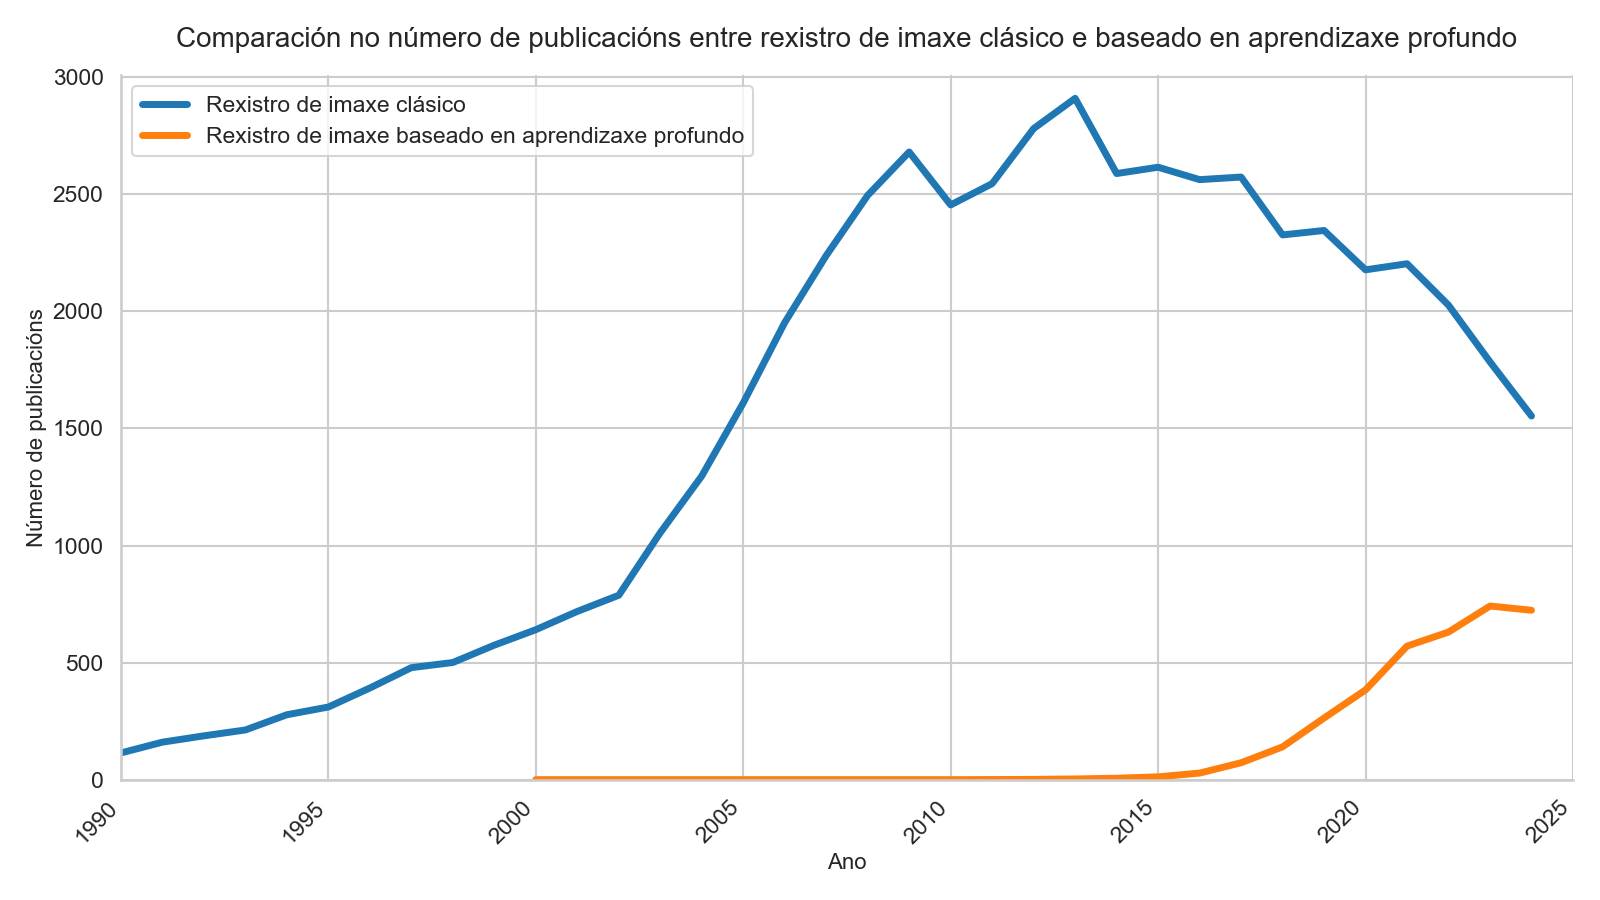
\includegraphics[width=0.8\textwidth]{imaxes/methods_comp.png}
\caption{Comparación de pubicacións ó longo do tempo que relacionadas co rexistro de imaxes. Datos extraídos de Scopus \cite{scopus}, realizando as consultas: "TITLE-ABS-KEY(image AND registration) AND NOT(deep AND learning)" e "TITLE-ABS-KEY(image AND registration) AND (deep AND learning)"}
\label{fig:method_comp}
\end{figure}

Os métodos de aprendizaxe profunda poden substituír calquera destes pasos que forman os métodos de rexistro clásicos de forma independente ou en combinación.

\paragraph{En rexistro baseado en intensidade (IBR)}
\label{par:IBR_substitution}

\begin{itemize}
\item \textbf{Métrica de similitude:} Os métodos de aprendizaxe profunda poden aprender métricas de similitude máis robustas que as tradicionais. Estas métricas aprendidas poden ser máis efectivas en imaxes multimodais ou con artefactos.
Por exemplo, Czolbe et al. \cite{semanticsimilarity} propoñen dúas métricas de similitude semánticas que aprende a semellanza entre imaxes comparando as características de alto nivel extraídas. Presentan unha aproximación non supervisada que fai uso de autoencoders e outra semisupervisada que incorpora datos de segmentación.
\item \textbf{Optimizador:} Os métodos de aprendizaxe profunda poden substituír o proceso de optimización iterativa tradicional por redes que aprenden a predicir directamente os parámetros de transformación óptimos. Unha aproximación común é empregar estes conxuntos de datos para optimizar unha CNN que, dadas dúas imaxes novas e non vistas, predí o DFV correspondente \cite{defregcnn}. Durante o proceso de adestramento, a rede pode ter acceso aos DFVs ca deformación correcta, ou pódense obter indirectamente a través da optimización dunha métrica de similitude de imaxes.
\item \textbf{Modelo de transformación:} Estes métodos aprenden representacións implícitas da transformación a través de redes neuronais, permitindo modelar deformacións máis complexas que os modelos paramétricos tradicionais. Os métodos como IDIR \cite{wolterink2021implicit} encaixan nesta categoría, utilizando campos neuronais implícitos para representar as transformacións de rexistro.
\end{itemize}

% Existen diferentes extensións a esta aproximación, como o uso de múltiples etapas ou o uso de redes adversarias durante o adestramento.

% Tamén se propuxeron métodos híbridos que combinan a optimización iterativa ca aprendizaxe profunda,
% entrenando unha CNN nova por cada parella de imaxes. Desta forma conséguese evitar a necesidade de grandes conxuntos de datos para o adestramento.

\paragraph{En rexistro baseado en características (FBR)}
\label{par:FBR_substitution}

\begin{itemize}
\item \textbf{Detectores de características:} As redes neuronais poden aprender a detectar puntos de interese máis robustos e repetibles que os detectores clásicos como \glossary{SIFT}. SuperPoint \cite{superpoint} introduce un detector de características baseado en redes neuronais que aprende a detectar puntos de interese e a describilos simultaneamente.
\item \textbf{Descriptores de características:} Os descriptores aprendidos mediante redes neuronais poden capturar información máis discriminativa, mellorando a precisión do emparellamento posterior. Estes métodos aprenden representacións que son invariantes a transformacións específicas do dominio.
\item \textbf{Emparellamento:} As redes neuronais poden aprender a realizar o emparellamento de características de forma robusta, especialmente en presenza de cambios de iluminación ou perspectiva. SuperGlue \cite{superglue} é un exemplo de modelo que aprende a emparellar puntos de interese detectados utilizando unha arquitectura baseada en atención para capturar as relacións entre os puntos.
\end{itemize}

\paragraph{Métodos de regresión directa}
\label{par:direct_regression}

A aprendizaxe profunda tenden a requerir dunha gran cantidade de datos para ser adestrados, o que pode ser unha desventaxa xa que en moitos casos non se dispoñen de bases de datos anotadas do tamaño necesario.

Os métodos de regresión directa aprenden a mapear directamente desde un par de imaxes ata os parámetros da transformación, sen necesidade de optimización iterativa nin extracción explícita de características.

Tamén son denominados métodos de inferencia amortizada debido á capacidade de realizar múltiples inferencias (rexistros) tras un único proceso de adestramento, en contraposición aos métodos tradicionais que requiren optimización individual para cada par de imaxes.
Estes enfoques son útiles pola súa eficiencia computacional na fase de inferencia. Voxelmorph \cite{Balakrishnan_2019voxelmorph} é un dos frameworks máis utilizados no rexistro de imaxes deformable, facendo uso de modelos baseado en \gls{CNN}s e que tamén permite incorporar información auxiliar (como segmentacións) se está dispoñible, mellorando así a precisión do rexistro.

Métodos como UDIR-Net \cite{undefreg} ou DIO \cite{Jena_2025} tamén implementan estas ideas.

% \paragraph{GANs}
% \label{par:GANs}

% As \gls{GAN} (Generative Adversarial Network) son un tipo de rede neuronal que consta de dous modelos que compiten entre si: un xerador e un discriminador. O xerador intenta crear datos falsos que sexan indistinguibles dos datos reais, mentres que o discriminador intenta distinguir entre os datos reais e os datos xerados. Este proceso de competición mellora iterativamente a calidade dos datos xerados e o criterio do discriminador.

% No contexto do rexistro de imaxes, as GANs poden ser utilizadas para aprender a transformación entre imaxes de forma non supervisada. O xerador pode ser adestrado para producir transformacións que aliñen a imaxe móbil coa imaxe fixa, mentres que o discriminador avalía a calidade do rexistro.
% Un exemplo de aplicación de GANs no rexistro de imaxes médicas é o traballo de Mahapatra et al. \cite{mahapatra2019ganbasedmedicalimage}, onde se propón un modelo de rexistro de imaxes baseado en GANs que demostrou ser efectivo tanto en retinas como con resonancias magnéticas cardiovasculares.

\subsubsection{Estado da arte no rexistro de retinografías}
\label{subsubsec:Estado_da_arte_no_rexistro_de_retinografías}

O rexistro de retinografías presenta un conxunto de desafíos únicos que o distinguen doutros dominios da imaxe médica.
Un dos principais obstáculos son as deformacións non ríxidas. Estas deformacións poden orixínarse pola proxección da superficie 3D curva da retina nunha imaxe 2D ou variacións na forma do ollo de cada paciente. Ademais, é frecuente atopar pares de imaxes con áreas de solapamento mínimas o que dificulta a identificación de correspondencias para o aliñamento. A isto súmanse as variacións de iluminación, contraste e cor entre imaxes capturadas en diferentes situacións, así como os cambios anatómicos inducidos por patoloxías, que alteran as estruturas utilizadas para o rexistro. 
Finalmente, a escaseza de conxuntos de datos públicos, especialmente para condicións ou poboacións específicas, supón unha barreira importante para o desenvolvemento de modelos de aprendizaxe supervisada.    

A dificultade para obter campos de deformación de referencia para o adestramento impulsou o desenvolvemento de marcos non supervisados. Estes modelos adéstranse optimizando unha función de perda baseada na similitude de imaxe entre a imaxe móbil deformada e a imaxe fixa, xunto cun termo de regularización sobre a suavidade da deformación. 

% A figura \ref{tab:retina_reg_comp} mostra unha análise comparativa revela un claro compromiso entre precisión e velocidade. Métodos clásicos como REMPE poden acadar unha alta precisión, pero son computacionalmente moi custosos (p. ex., 198 segundos por par de imaxes). En contraste, os métodos de aprendizaxe profunda son ordes de magnitude máis rápidos (p. ex., 0.65 segundos por par), aínda que poden sacrificar parte da precisión nos casos máis complexos. A seguinte táboa resume esta comparativa.  

Dentro dos métodos clásicos, os baseados en características (FBR) seguen a ser referentes en canto a precisión. Entre eles destacan VOTUS \cite{Votus}, que é especialmente robusto en imaxes de pouco solapamento e representa as árbores vasculares como grafos para atopar a correspondencia entre eles. REMPE \cite{rempe} é outro método xa mencionado anteriormente nesta categoría.

No campo da aprendizaxe profunda, RetinaRegNet \cite{sivaraman2024retinaregnetzeroshotapproachretinal} é un modelo recente que de tipo "zero-shot" que utiliza características extraídas de modelos de difusión para establecer correspondencias, acadando resultados de vangarda

%  \cite{ConKeD}  \cite{ConKeD2}
ConKeD (Contrastive Keypoint Descriptors) e a súa evolución, ConKeD++ , céntranse en perfeccionar a creación de descritores de puntos de interese, un dos compoñentes máis críticos dos métodos baseados en características (FBR).
A principal vantaxe é que obtén resultados comparables aos dos métodos clásicos de vangarda (como REMPE e VOTUS) pero con tempos de execución moito máis rápidos

A maioría destes algoritmos son avaliados e comparados utilizando o conxunto de datos de referencia FIRE \cite{FIRE}, permitindo unha cuantificación obxectiva do rendemento.

\section{Representación Neuronais Implícitas}
\label{sec:Representación Neuronais Implícitas} 

A representación de coñecemento é un dos problemas máis importantes na área da computación, e as 
redes profundas son unha das ferramentas máis útiles, especialmente no campo da visión por computador.
Tradicionalmente empréganse representacións discretas, onde o espazo de entrada é dividido en celdas e cada celda é asignada un valor (por exemplo nubes de puntos, matrices de píxeles ou vóxeles...).
Unha das principais desventaxas destas representacións é que a súa complexidade increméntase rápidamente co número de dimensións representadas, ademais do custo de memoria asociado.

 As representacións neuronais implícitas son un paradigma innovador que permite modelar sinais continuas mediante funcións parametrizadas por redes neuronales.
 Codifican a información como unha función continua, que mapea valores de entrada aos valores correspondientes de saída, en lugar de almacenar directamente valores de características o señales.

Representar o sinal como una función continua permite solucionar os problemas asociados á discretización e obtéñense outra serie de vantaxes.

As INR son moito mais eficientes debido á compresión da información que realizan de forma implícita. Ao mesmo tempo, permite un nivel de detalle non limitado pola resolución da imaxe, senón pola capacidade da rede. 
 Ademais, as representacións continuas son diferenciables, o que permite o cálculo de gradientes e derivadas de forma analítica en lugar de ter que aproximalos por diferencias finitas.
 Isto tamén implica que as representacións implícitas son independentes da resolución, o que permite a reconstrucción en calquera escala espacial.
 
Tipicamente emprégase un MLP como architectura para representar a función implícita. Non obstante, o uso da función de activación ReLU tende a non obter os mellores resultados, debido a que son incapaces de representar deformacións locais sen afectar o sea comportamento global \cite{rahaman2019spectralbiasneuralnetworks},
polo que moita investigación diríxese a atopar alternativas que melloren a representación do sinal. \cite{essakine2024standimplicitneuralrepresentations}

Unha destas alternativas é SIREN \cite{sitzmann2020implicitneuralrepresentationsperiodic}, sobre a que profundizaremos máis adiante.
Outras propostas inclúen \cite{ramasinghe2022periodicityunifyingframeworkactivations} propón as funcións de activación gaussianas como alternativa a SIREN, e argumenta que poden obter mellores representacións e máis robustas.
\cite{saragadam2023wirewaveletimplicitneural} achega unha nova función de activación baseada en wavelets, que parece ser especialmente útil para a representación de imaxes.

As representacións implícitas poden ser clasificadas en dúas categorías: xeneralizables e sobreaxustadas \cite{yu2024neuraltrajectorymodelimplicit}. 
As representacións sobreaxustadas céntranse en reproducir con precisión unha única sinal, mentres que as representacións xeneralizables poden modelar varias nunha mesma rede.

\subsection{Aplicacións}
\label{subsec:Aplicacións}

As INR son utilizadas en todo tipo de campos, dende xeración de imaxes \cite{reddy2022multiimplicitneuralrepresentationfonts}, pasando por
reconstrucción de obxetos \cite{mildenhall2020nerfrepresentingscenesneural} \cite{mescheder2019occupancynetworkslearning3d} ou modelado de sinais complexas \cite{wu2021iremhighresolutionmagneticresonance}.

As representacións implícitas están a recibir cada vez máis atención da comunidade médica, e son 
especialmente útiles para as tarefas de imaxe inversa, que requiren a reconstrucción de representacións correctas a partir de datos incompletos ou ruidosos \cite{molaei2023implicitneuralrepresentationmedical}. 
Métodos como NeRP, propuxeron o uso de representacións implícitas para a reconstrucción de imaxes de resonancia magnética a partir de datos incompletos, 
e obtiveron resultados comparables a métodos tradicionais \cite{shen2023nerpimplicitneuralrepresentation}.

NeRF fai uso de representacións implícitas para a sintetizar novos puntos de vista en escenas 3D  \cite{mildenhall2020nerfrepresentingscenesneural}, 
 optimizando unha función volumétrica continua que modela a densidade de volume e a radiancia emitida en cada punto do espazo.
 Utilizan un MLP, cuxa entrada é unha única coordenada continua 5D (localización espacial (x, y, z) e dirección de visión (θ, φ)) 
 e cuxa saída é a densidade de volume e a radiancia emitida dependente da vista nesa localización espacial. 
A única entrada necesaria para optimizar a súa representación é un conxunto de imaxes con poses de cámara coñecidas. 
Este traballo demostra que as representacións implícitas están capacitadas para modelar escenas 3D complexas con alta fidelidade visual.
 
As representacións implícitas tamém teñen bastante potencial no campo de planificación de traxectorias, 
onde se fai uso de INRs para modelar entornos e planificar traxectorias para un ou varios axentes \cite{yu2024neuraltrajectorymodelimplicit}.
A principal vantaxe de facelo desta forma frente á forma tradicional (algoritmos computacionalmente intensos, especialmente para multi-axentes) é a velocidade á que encontran solucións (por debaixo do milisegundo en GPUs).
A maior desventaxe é que non garanten a converxencia a unha solución óptima e sen colisións, mais os autores demostran que a calidade das traxectorias xeradas é adecuada para a maioría das aplicacións \cite{trajectinr}.

No ámbito médico, utilizanse este tipo de representacións para garantir a seguridade do paciente durante a cirurxía teleoperada e optimizar a traxectoria do robot para evitar colisións co paciente, por exemplo nas boca e gorxa \cite{teleoperatdrob}.
Con este método, evítase a reconstrución de mallas a partir de imaxes, que é un proceso costoso e imperfecto, e modélase mediante unha INR a partir dos datos médicos dispoñibles.
Os comandos de movemento da man do operador son tomados como entrada polo modelo, que logo de un proceso de optimización, xera unha secuencia de movementos libre de colisións que será enviada á man robótica.
Tamén son utilizadas para crear reconstruccións 3D de pulmóns que mitigan as distorsións causadas polo movemento respiratorio \cite{velikova2024implicitneuralrepresentationsbreathingcompensated}.

Outro uso interesante das representacións neuronais implícitas é a compresión de imaxes. Algoritmos como COIN \cite{coin} representan os datos de entrada mediante redes neuronais implícitas (funcións que mapean coordenadas a valores RGB), logrando unha compresión eficiente e unha redución significativa do tempo de codificación en moitas modalidades.

\subsection{Rexistro baseado en Representacións Neuronais Implícitas}
\label{subsec:Rexistro_baseado_en_INRs}

O rexistro de imaxes baseado en Representacións Neuronais Implícitas (INR) parametriza a transformación de deformación como unha función continua, xeralmente cun Perceptrón Multicapa (MLP), que mapea coordenadas espaciais a vectores de desprazamento. A diferenza das CNN, a rede non procesa as intensidades da imaxe directamente, senón que se optimiza usando estas para calcular a perda. Unha das vantaxes neste contexto é a capacidade de calcular gradientes analíticos exactos da transformación, permitindo unha regularización máis precisa que con aproximacións dos métodos baseados en grellas.  

As funcións de activación periódicas (SIREN \cite{sitzmann2020implicitneuralrepresentationsperiodic}) permitiron sobrepasar o problema dos sesgos cara transformacións de baixa frecuencia do MLP, e foron utilizadas por IDIR acadando resultados de vangarda \cite{wolterink2021implicit}.  

Os principais inconvenientes son a lentitude na inferencia (require optimización para cada par de imaxes) e a tendencia a xerar pregamentos espaciais (deformacións non realistas). A investigación actual céntrase en modelos híbridos para mitigar estes problemas.
Algúns dos enfoques máis relevantes inclúen:
SINR (Spline-enhanced INR) combina INR con B-splines, onde a rede predí os desprazamentos dunha grella de control dispersa. Isto impón suavidade de forma intrínseca e facilita o rexistro multimodal \cite{SINR}.   
INR ciclo-consistentes, que adestran simultaneamente a transformación directa e a inversa, usando cada rede como regularizador da outra para mellorar a robustez.  
Meta-aprendizaxe: Aprende unha inicialización de pesos óptima a partir dun gran conxunto de datos para acelerar drasticamente a converxencia na inferencia \cite{learnedinit}.  
INR condicionadas por xeometría: Incorporan coñecemento anatómico previo para simplificar a complexidade da deformación a aprender \cite{harten2023deformable}.  
Sun et al. \cite{sun2024medicalimageregistrationneural} propóñen un rexistro de imaxes que usa campos neuronais para modelar a transformación, utilizando tamén codificación posicional (que transforma a coordenadas espaciais en vectores de alta dimensión) o que permite que a rede aprenda con maior facilidade as transformacións de alta frecuencia.

O uso de Representacións Neuronais Implícitas (INR) para o rexistro de imaxes ofrece unha precisión notable ao modelar a deformación como unha función continua e analiticamente diferenciable. Este enfoque, exemplificado polo éxito inicial de IDIR, permite unha regularización máis exacta que os métodos baseados en grellas. Non obstante, a súa aplicación práctica vese obstaculizada pola lentitude da optimización por cada par de imaxes e o risco de producir deformacións non realistas con pregamentos espaciais. O estado da arte actual tende a abordar estes retos mediante a hibridación.

\section{Traballo proposto}
\label{sec:Traballo proposto}

O traballo proposto ubícase dentro do dos métodos de aprendizaxe profunda, e máis concretamente no rexistro de imaxes baseado en intensidade (IBR) utilizando representacións neuronais implícitas (INRs).

Como mostramos neste capítulo, a pesar do potencial das representacións neuronales implícitas en diversos dominios médicos, a súa aplicación específica ao rexistro de retinografías permanece inexplorada.

Este falta de investigación é especialmente relevante dadas as potenciais vantaxes que ofrecen as INRs, como a capacidade de modelar deformacións complexas e a súa independencia da resolución.

Baseándose no framework introducido por \cite{wolterink2021implicit}, propónse modificalo para adaptalo á tarefa de rexistro de retinografías. O obxetivo é conseguir rexistros consistentemente precisos, especialmente no dataset de FIRE que contén imaxes reais de retina.

Esta adaptación representa unha contribución novel ao estado da arte no rexistro de retinografías, explorando por primeira vez o potencial das representaciones neuronales implícitas neste dominio específico.
